\documentclass[a4paper,10pt]{article}
\usepackage[utf8x]{inputenc}

\usepackage[left=2.5cm,right=2.5cm,top=2cm,bottom=2cm]{geometry}
\usepackage{amsmath,amsfonts,amssymb}
\usepackage{graphicx}
\usepackage[colorlinks=true,linkcolor=blue,urlcolor=blue,citecolor=blue]{hyperref}
\usepackage{color}
\usepackage{listings}

%opening
\title{PicoHarp300 Device Server}
\author{Sergi Blanch-Torn\'e\\\small{Controls Software Engineer - Alba Synchrotron}\\{\tt \small{sblanch@cells.es}}}

\newcommand{\todo}[1]{\texttt{\color{red}TODO:} ``\emph{#1}''}
\newcommand{\fixme}[1]{\texttt{\color{red}FIXME:} ``\emph{#1}''}
\newcommand{\ok}[1]{``#1'' [\texttt{\color{green}OK}]}

\begin{document}

\maketitle

\begin{abstract}
\todo{...}
\end{abstract}

\section{Python extension}

\todo{cython}

\section{Device design}

\todo{...}

\subsection{Machine state}

\begin{figure}[h]
    \centering{
         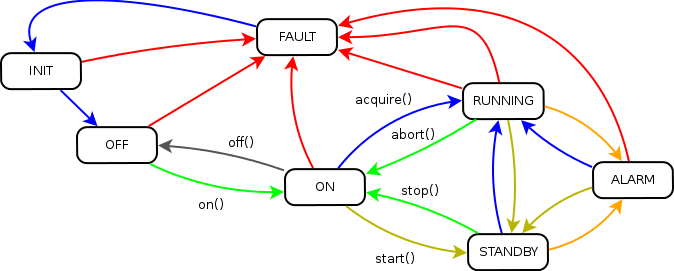
\includegraphics[width=0.75\textwidth]{StateMachine.png}
         \caption{State machine diagram of the Device in the Skippy Device Server} \label{fig:stateMachine}
    }
\end{figure}

\todo{explain the figure \ref{fig:stateMachine}}

\subsection{Device Properties}

\begin{itemize}
    \item {\tt SerialNumber}: \todo{...}
    \item {\tt Simulation}: optional property \todo{...}
\end{itemize}

\subsection{Device Commands}

\begin{itemize}
    \item {\tt Off()}: \todo{...}
    \item {\tt On()}: \todo{...}
    \item {\tt Start()}: \todo{...}
    \item {\tt Stop()}: \todo{...}
    \item {\tt Acquire()}: \todo{...}
    \item {\tt Abort()}: \todo{...}
    \item {\tt \emph{Exec():}} Expert attribute to look inside the device during execution.
\end{itemize}

\subsection{Device Attributes}

\begin{itemize}
    \item {\tt InstrumentModel}: \todo{...}
    \item {\tt InstrumentPartnum}: \todo{...}
    \item {\tt InstrumentVersion}: \todo{...}
    \item \todo{...}
\end{itemize}

\subsection{Uml Diagrams}

In figure \ref{fig:classDiagram} can be found a UML draw with the class diagram.

\begin{figure}[h!]
    \centering{
         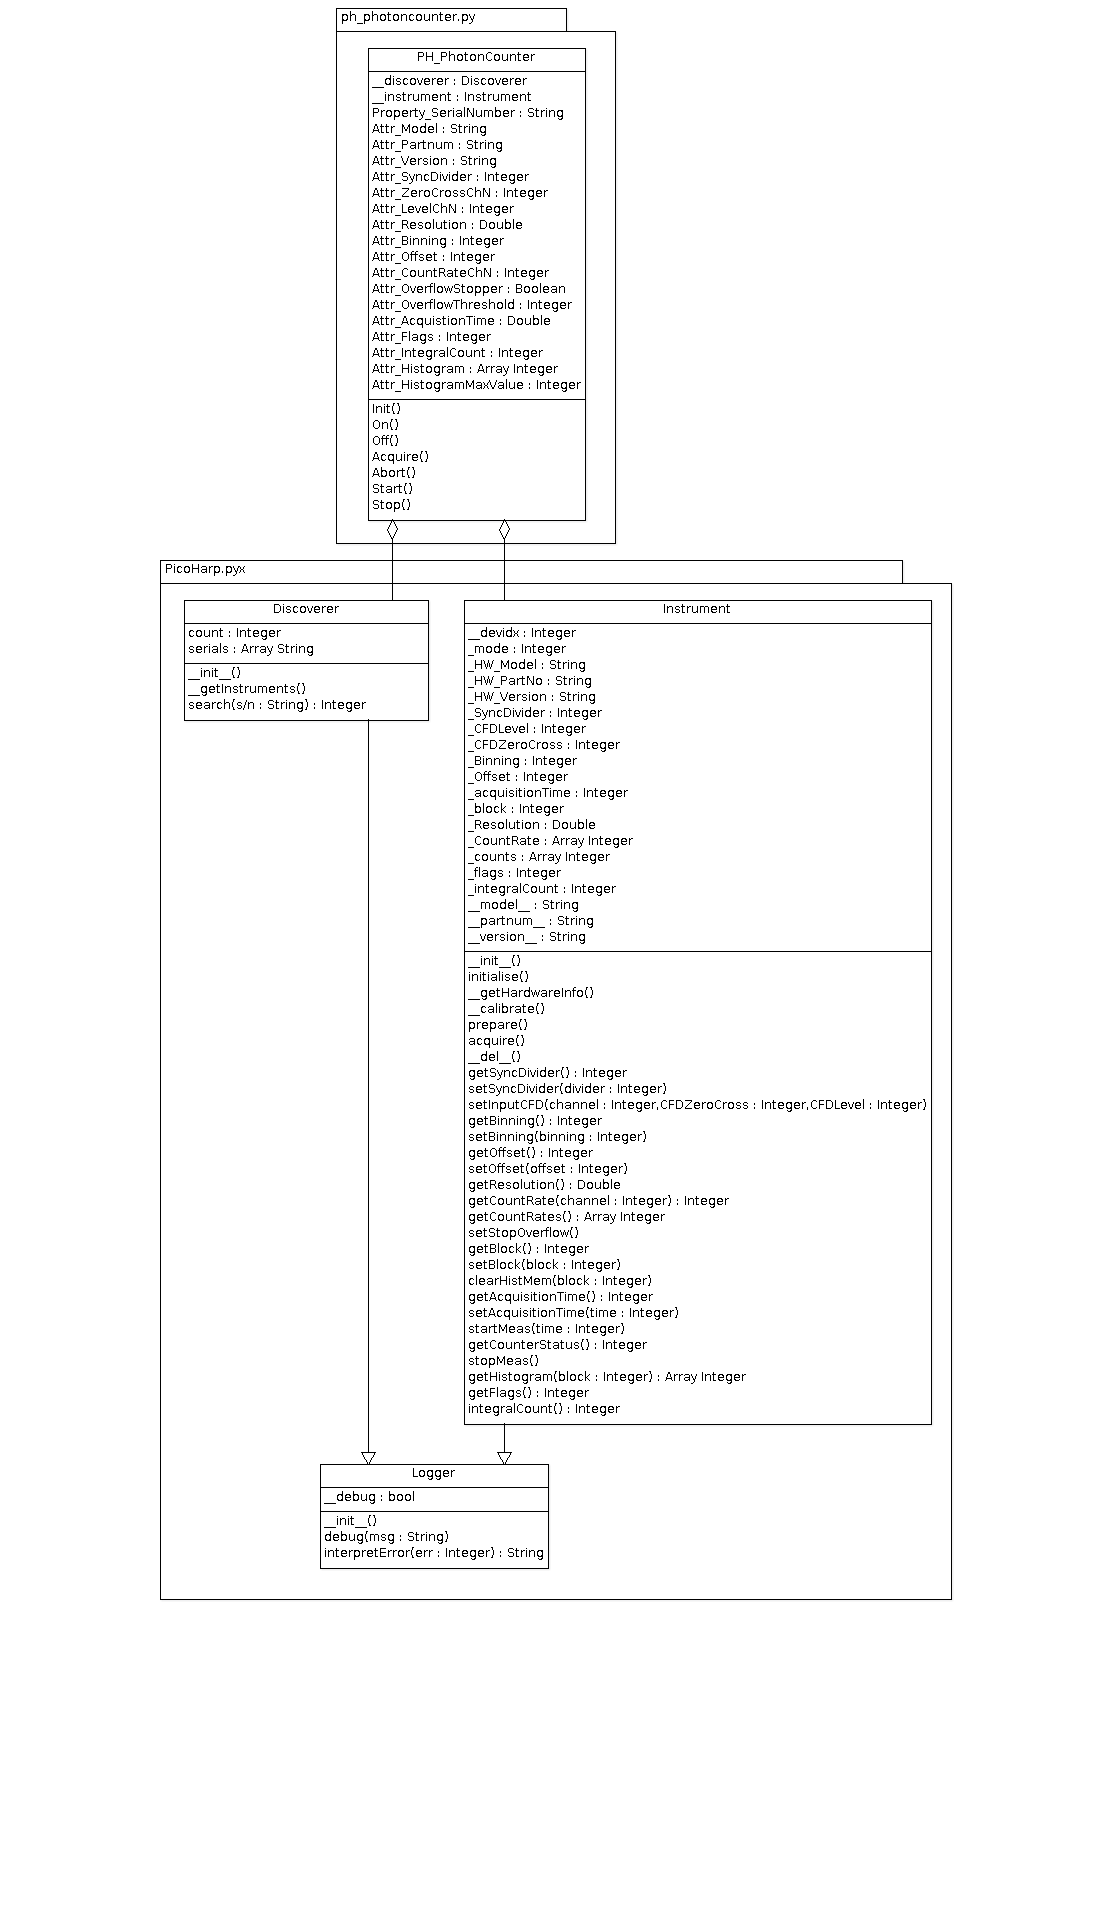
\includegraphics[width=\textwidth]{ClassDiagram_PicoHarp.png}
         \caption{Class diagram of the PicoHarp.} \label{fig:classDiagram}
    }
\end{figure}

\begin{figure}[h!]
    \centering{
         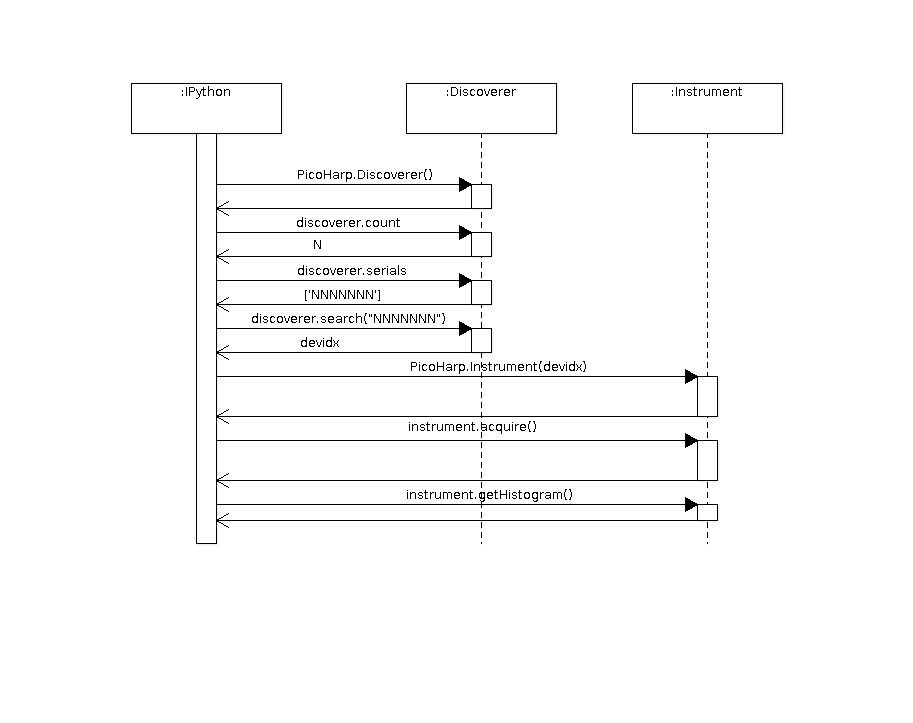
\includegraphics[width=\textwidth]{CollaborationDiagram_PicoHarp.png}
         \caption{Collaboration diagram of the PicoHarp.so} \label{fig:classDiagram}
    }
\end{figure}

\subsection{Device features}

\todo{...}

%\subsection{Known bugs}

\section{Taurus graphical user interface}

\todo{...}

\end{document}
